\documentclass[11pt]{article}

\usepackage[margin=2.5cm]{geometry}
\usepackage{amsmath}
\usepackage{amssymb}
\usepackage{graphicx}
\usepackage{float}
\usepackage{booktabs}
\usepackage{array}
\usepackage{tabularx}
\usepackage{hyperref}

\title{Model-Based vs.\ Model-Free Reinforcement Learning:\\
Value Iteration and Q-Learning on the Stochastic Windy Gridworld}
\author{Tanzila Khan \\ Roll - 25}
\date{}

\begin{document}
\maketitle

\section{Objective}

This lab compares a model-based method (Value Iteration) with a model-free
method (Q-Learning) on the same Markov Decision Process and examines how
their hyperparameters behave. The environment is the \textbf{Stochastic
Windy Gridworld}, a grid-world navigation task with a column-dependent,
stochastic crosswind, implemented as a custom Gymnasium environment.

Windy Gridworld is multi-step, delayed-reward, and stochastic through a
column-dependent wind. This combination is what lets $\gamma$ change the
optimal \emph{policy} itself here, rather than only the speed of
convergence (Section~8.1). Most states (64 of 69) also have a clearly best
action with a real margin over the runner-up (Section~7), so Q-Learning is
expected to recover Value Iteration's policy on almost all of them.

\section{Environment}

A $7\times10$ grid. The agent starts at $S=(3,0)$
(row, column) and must reach the goal $G=(3,7)$. Four actions are available:
UP, DOWN, LEFT, RIGHT, each moving one cell (clipped at the grid edge). The
wind strength used for a move is read from the column the agent
\emph{occupies before} the move (the standard convention), and the resulting
row shift is applied to the landing column:

\begin{center}
\begin{tabular}{lcccccccccc}
column & 0 & 1 & 2 & 3 & 4 & 5 & 6 & 7 & 8 & 9 \\
mean wind & 0 & 0 & 0 & 1 & 1 & 1 & 2 & 2 & 1 & 0 \\
\end{tabular}
\end{center}

In a windy column (mean wind $w>0$), the \emph{actual} push each time the
agent passes through is stochastic: $w-1$, $w$, or $w+1$, each with
probability $1/3$; calm columns push deterministically by $0$. All
positions are clipped to the grid.

\begin{itemize}
  \item \textbf{State:} \texttt{(row, col)}, a genuine Markov state, since
        the wind at a column is drawn i.i.d.\ every time the agent passes
        through it. The model has 69 non-terminal states (the goal is
        absorbing).
  \item \textbf{Actions:} \texttt{0=UP, 1=DOWN, 2=LEFT, 3=RIGHT}
        (\texttt{Discrete(4)}).
  \item \textbf{Reward:} $-1$ on every transition, including the one that
        reaches the goal, which ends the episode.
\end{itemize}

\begin{figure}[H]
\centering
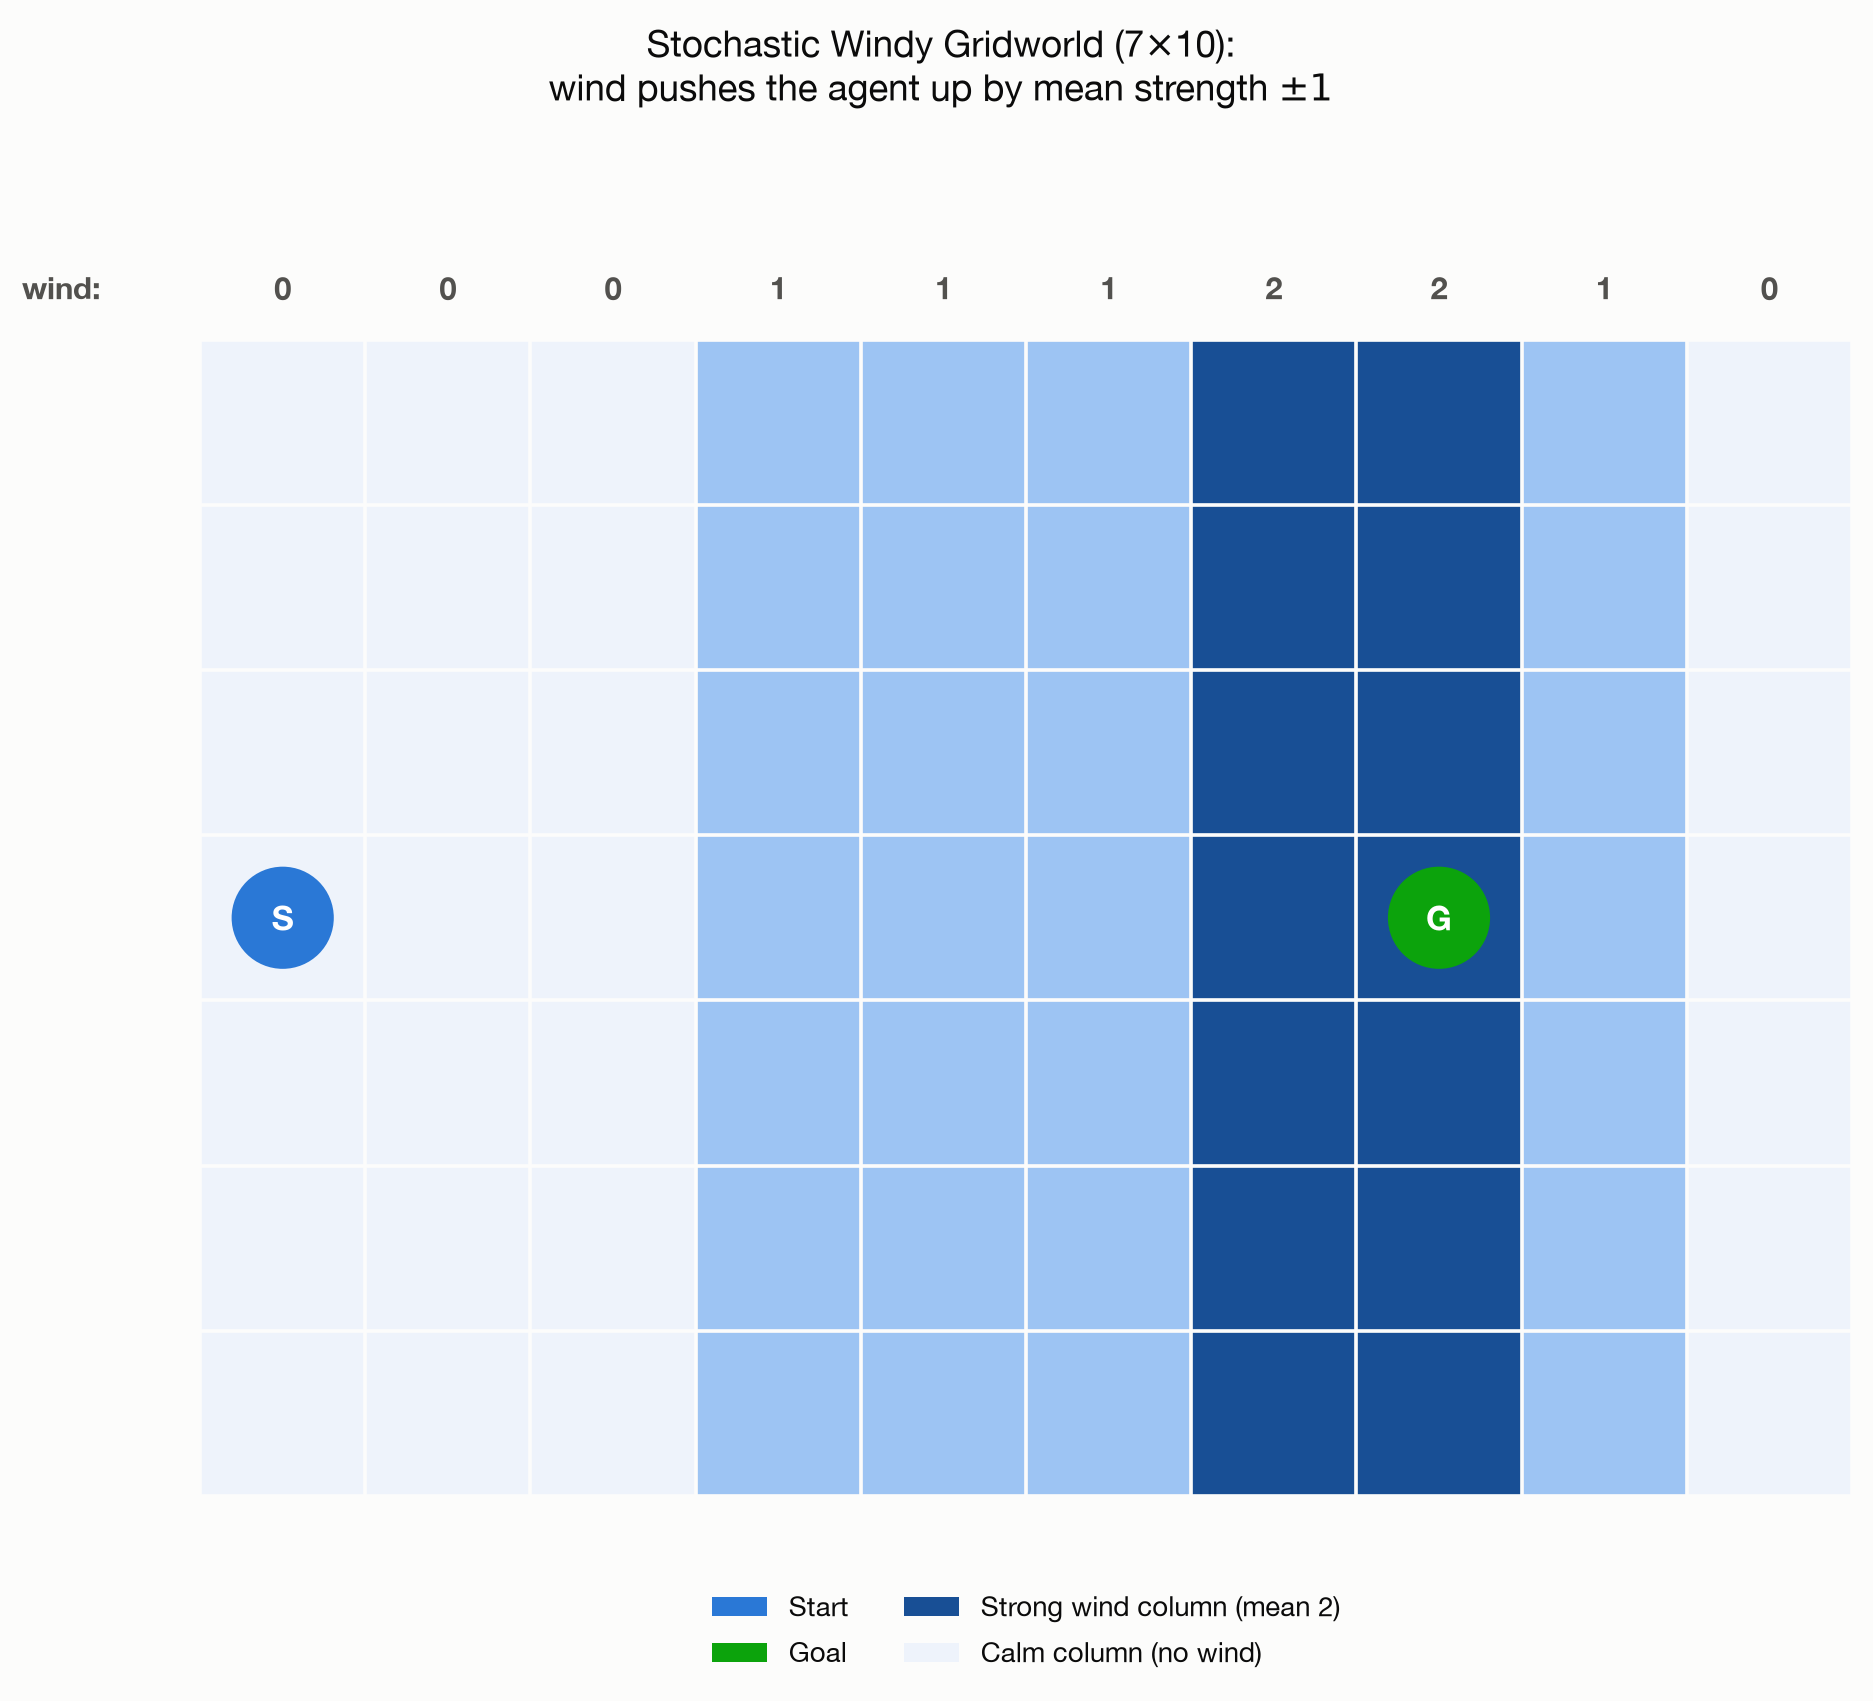
\includegraphics[width=0.75\textwidth]{fig_environment.png}
\caption{The Stochastic Windy Gridworld. Darker columns carry stronger mean
wind; the wind's actual strength on any single pass varies by $\pm1$.}
\label{fig:env}
\end{figure}

\section{Theoretical Grounding}

Both algorithms compute the same object. Under the \textbf{principle of
maximum expected utility (MEU)}, a rational agent chooses the action
maximising
$$EU(a) = \sum_{s'} P(\text{RESULT}(a)=s')\,U(s').$$
Value Iteration computes exactly this at each state from the derived
wind model. The \textbf{Markov property} (Section~2) makes the
\textbf{Bellman equation}
$$U(s) = \max_a \sum_{s'} P(s'\mid s,a)\big[R(s,a,s') + \gamma\, U(s')\big]$$
well defined; Value Iteration solves it by repeated Bellman updates,
Q-Learning estimates the same right-hand side online with learning rate
$\alpha$, sampling transitions from the real environment instead of summing
over a known model. In the course's classification, both methods are
\emph{value-based}, and Q-Learning is \emph{off-policy}: its update
bootstraps off $\max_a Q(s',a)$ regardless of the exploratory action actually
taken.

\paragraph{Why $\gamma$ matters here.} With reward $-1$ per step
until an absorbing goal, the discounted return from a state under a fixed
number of remaining steps $T$ is $-\,\frac{1-\gamma^T}{1-\gamma}$, which as a
function of the step count $T$ is decreasing and convex (equivalently, the
accumulated cost $\frac{1-\gamma^T}{1-\gamma}$ is increasing and concave in
$T$). In a \emph{deterministic} shortest-path problem,
each fixed policy induces a fixed completion time $T$, so any $\gamma\in(0,1)$ ranks policies
identically: $\gamma$ only has to be strictly less than 1. Here $T$ is a
\emph{random variable} (the wind), so a policy's value is
$\mathbb{E}\!\left[-\frac{1-\gamma^T}{1-\gamma}\right]=-\frac{1-\mathbb{E}[\gamma^T]}{1-\gamma}$,
which by Jensen's inequality depends on the whole distribution of $T$ through
$\mathbb{E}[\gamma^T]$, not only its mean. The value of $\gamma$ sets how
heavily the tail of the step-count distribution is weighted and can change
which policy is optimal. Section~8.1 shows this is not a theoretical curiosity: at
$\gamma=0.7$ the greedy policy is different from $\gamma\ge0.9$'s,
not merely slower to compute.

\section{Deriving the Transition Model}

Because Windy Gridworld is a custom environment, Gymnasium exposes no
transition table, so the model is derived analytically from the wind's known
probabilities. From state \texttt{(r, c)} taking action
$a$: the deterministic part of the move gives an intermediate cell
\texttt{(r1, c1)} (clipped to the grid). Wind strength is determined by the
pre-action column \texttt{c}, not the landing column \texttt{c1}: if column
\texttt{c} is calm, the wind push is deterministically $0$; if it carries
mean wind $w>0$, the push is $w-1$, $w$, or $w+1$ each with probability
$1/3$. That row shift is then applied to the landing column: the next state
is \texttt{(r1 - push, c1)}, clipped to the grid, with reward $-1$ and the
episode ending if that cell is the goal.

\section{Value Iteration}

\paragraph{Algorithm.} Value Iteration turns the Bellman optimality equation
(Section~3) into a synchronous update rule, applied to every state until the
value function stops changing appreciably:
\begin{enumerate}
  \item \textbf{Initialise} $V_0(s) = 0$ for every non-terminal state $s$;
        $V(s_{\text{goal}}) = 0$, fixed, since the goal is absorbing.
  \item \textbf{Repeat} for sweep $k = 1, 2, \dots$:
  \begin{enumerate}
    \item For every non-terminal state $s$ and every action $a$, compute the
          action value under the current estimate, using the transition
          model derived in Section~4:
          $$Q_k(s,a) = \sum_{s'} P(s'\mid s,a)\big[R(s,a,s') + \gamma\, V_{k-1}(s')\big]$$
    \item Update the state value greedily: $V_k(s) = \max_a Q_k(s,a)$.
    \item Track the largest change across all states,
          $\Delta_k = \max_s \lvert V_k(s) - V_{k-1}(s)\rvert$.
  \end{enumerate}
  \item \textbf{Stop} once $\Delta_k < \theta$.
  \item \textbf{Extract} the greedy policy from the converged $V^*$:
        $$\pi^*(s) = \arg\max_a \sum_{s'} P(s'\mid s,a)\big[R(s,a,s') + \gamma\, V^*(s')\big]$$
\end{enumerate}

Value Iteration was run with $\gamma=0.99$ and threshold $\theta=10^{-10}$;
it converges in \textbf{116 sweeps} (Figure~\ref{fig:convergence}). Rolled
out from the start for 5{,}000 episodes (evaluation seed 1), the greedy policy reaches the goal
every time, in 20.53 steps on average. Figure~\ref{fig:value} shows
the resulting value function: $V^*(s) = -$(expected discounted steps to the
goal), lowest (most negative) far from the goal and in the strong-wind
columns, where the stochastic overshoot is costliest to correct.

\begin{figure}[H]
\centering
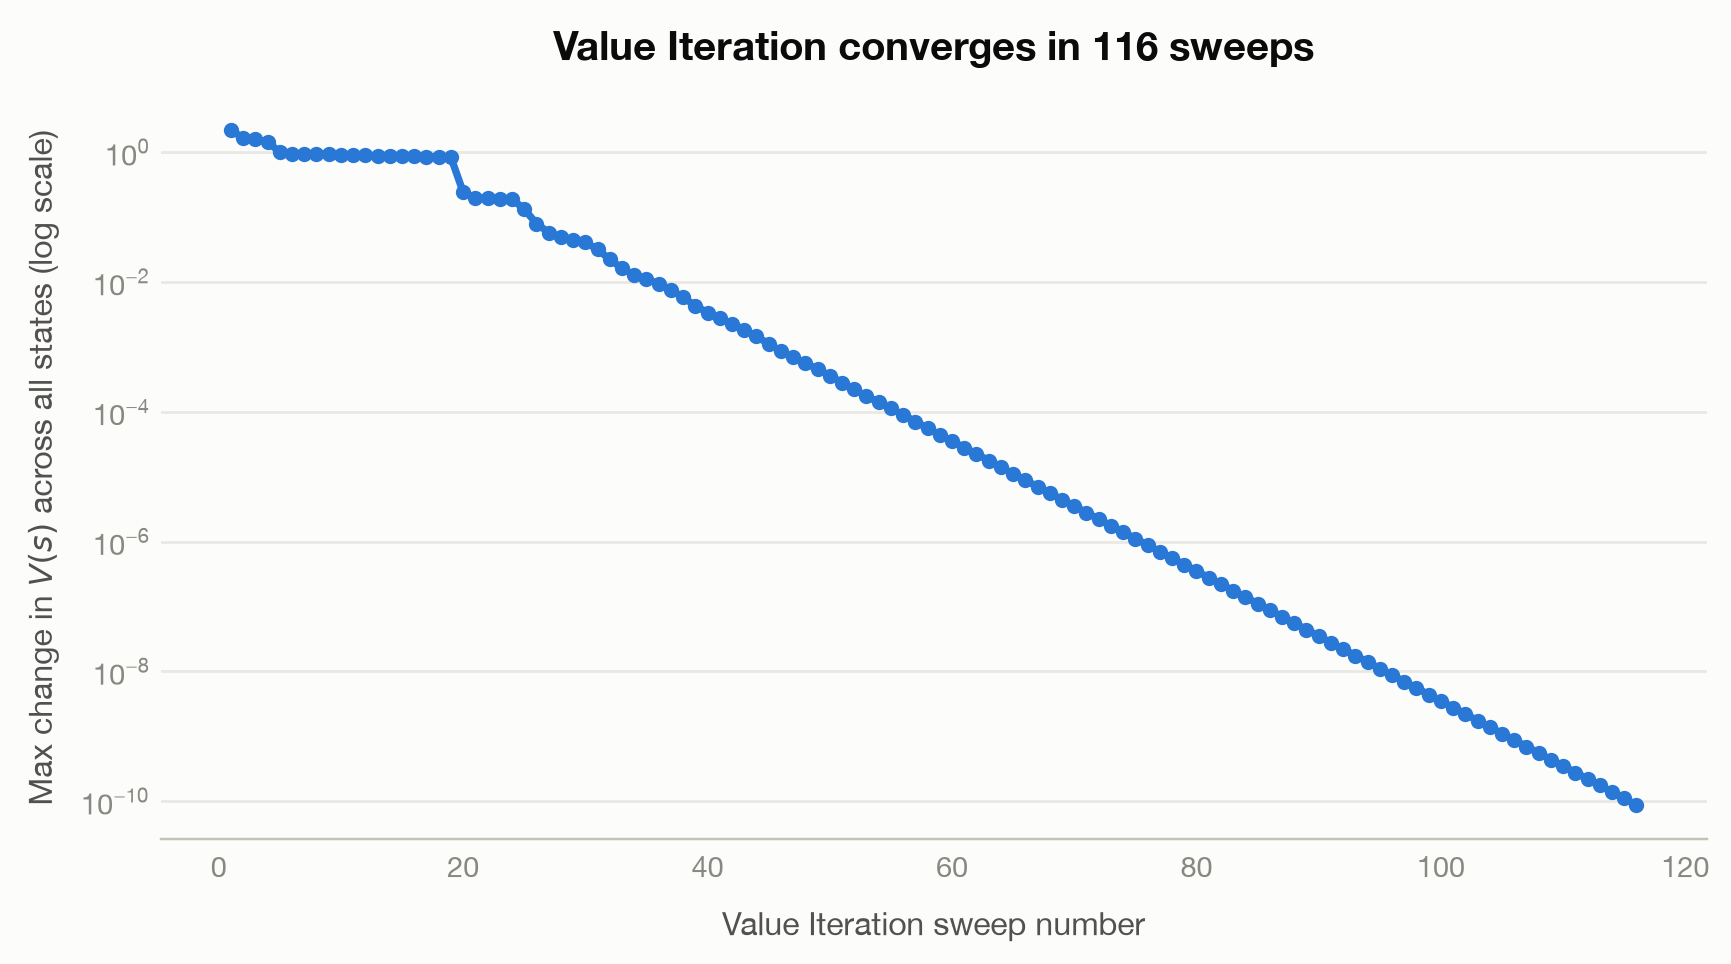
\includegraphics[width=0.62\textwidth]{fig_vi_convergence.png}
\caption{Value Iteration convergence.}
\label{fig:convergence}
\end{figure}

\begin{figure}[H]
\centering
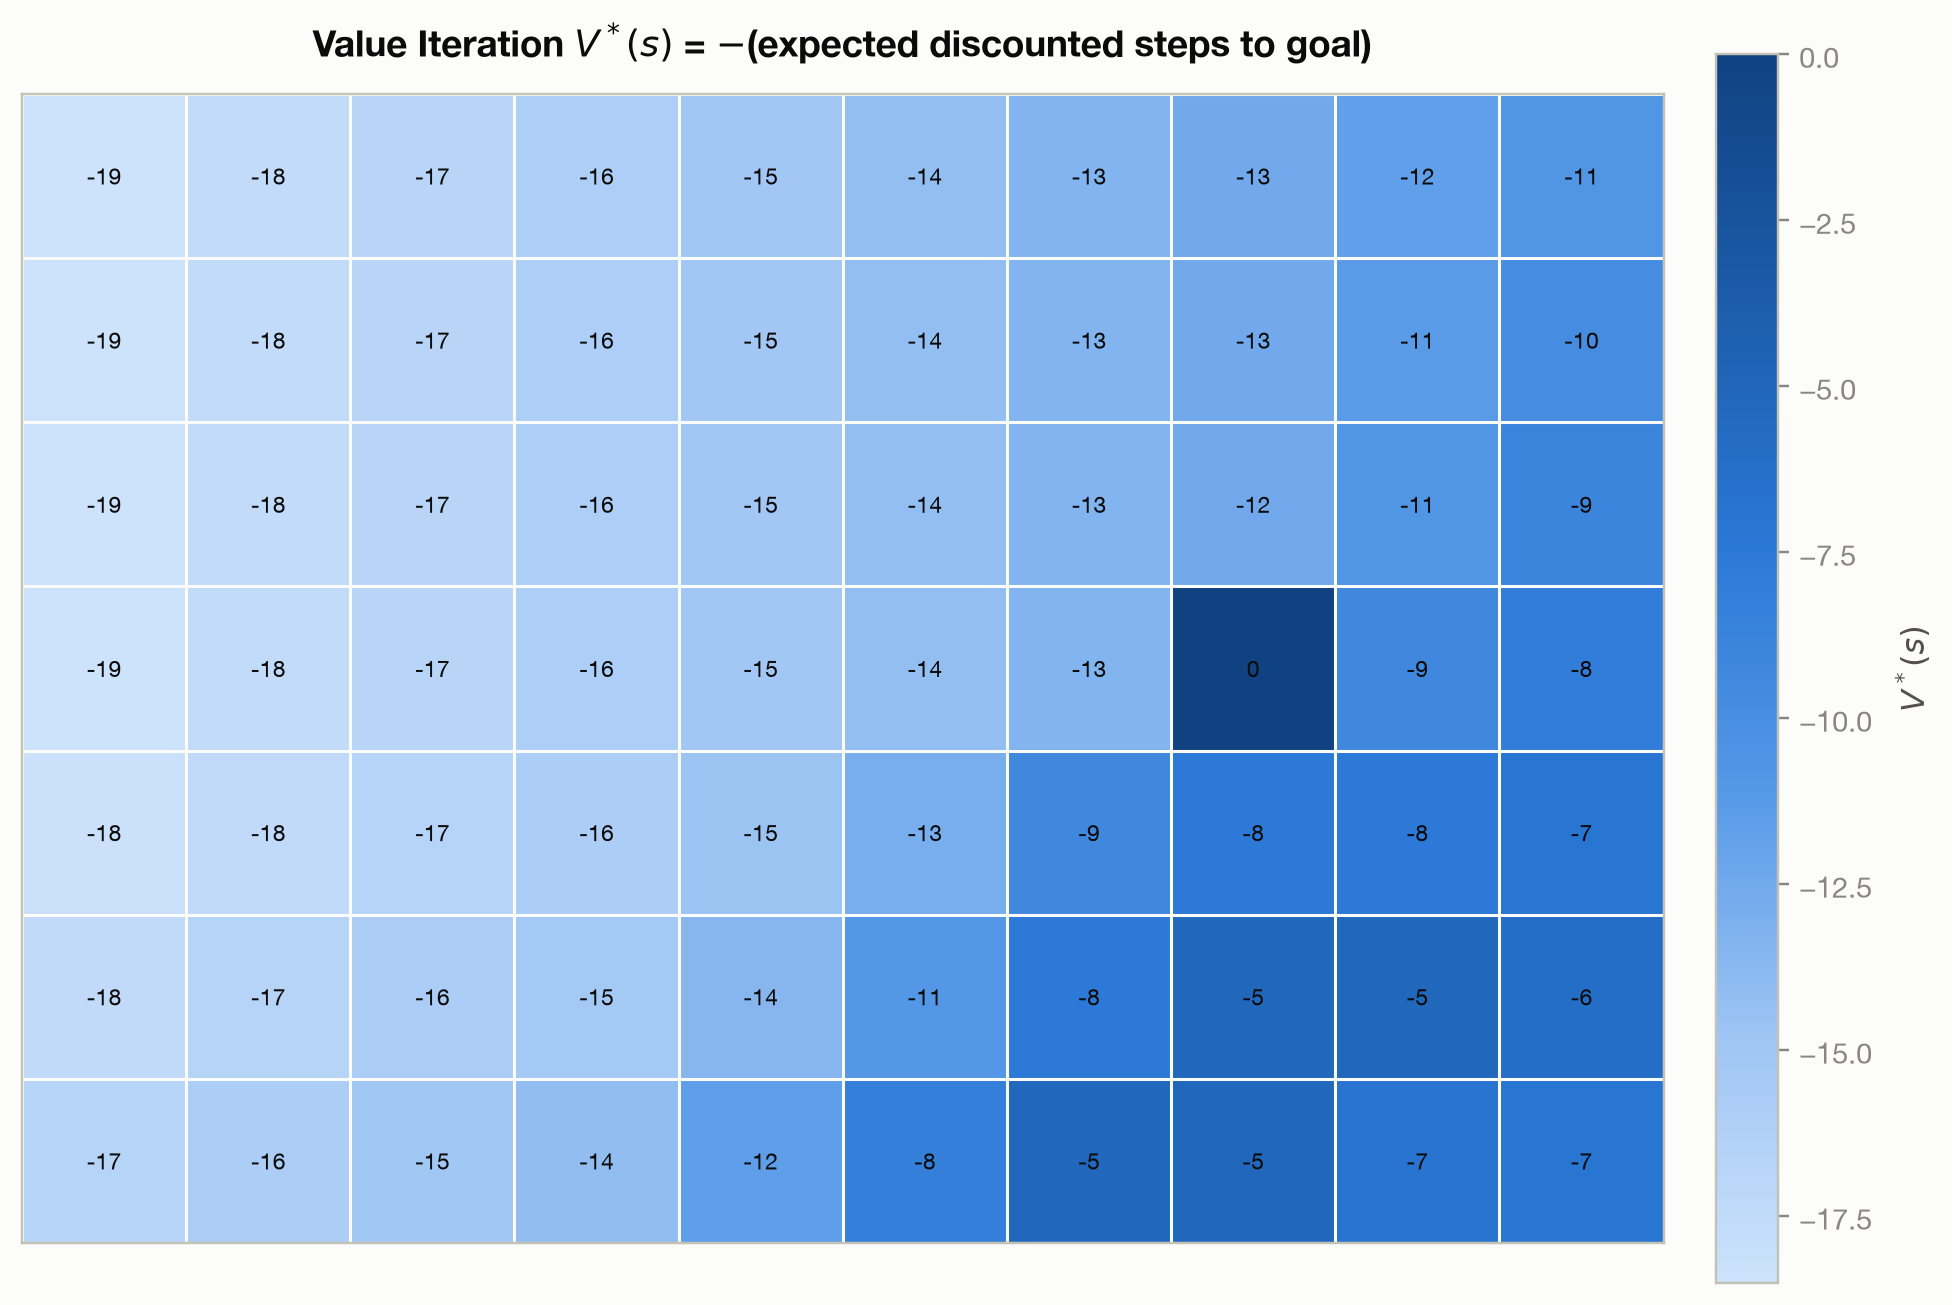
\includegraphics[width=0.68\textwidth]{fig_value_heatmap.png}
\caption{$V^*(\text{row}, \text{col})$ over the grid.}
\label{fig:value}
\end{figure}

\section{Q-Learning}

\paragraph{Algorithm.} Q-Learning estimates the same Bellman optimality
equation without a transition model, by sampling transitions from the real
environment and bootstrapping off its own current estimate:
\begin{enumerate}
  \item \textbf{Initialise} $Q(s,a) = 0$ for every state-action pair; set the
        exploration rate $\varepsilon = \varepsilon_0$.
  \item \textbf{For each episode:}
  \begin{enumerate}
    \item Initialise the state $s$ at the fixed start.
    \item \textbf{Repeat} for each step until $s$ is terminal:
    \begin{enumerate}
      \item Choose action $a$ from $s$ using an $\varepsilon$-greedy policy
            over $Q(s,\cdot)$: the greedy action $\arg\max_a Q(s,a)$ with
            probability $1-\varepsilon$, a uniformly random action otherwise.
      \item Take action $a$ via \texttt{env.step(a)}; observe reward $r$ and
            next state $s'$.
      \item Update the estimate toward the sampled Bellman target:
            $$Q(s,a) \leftarrow Q(s,a) + \alpha\Big[r + \gamma\max_{a'} Q(s',a') - Q(s,a)\Big]$$
      \item $s \leftarrow s'$.
    \end{enumerate}
    \item Decay $\varepsilon$ toward its floor.
  \end{enumerate}
  \item \textbf{Extract} the greedy policy: $\pi(s) = \arg\max_a Q(s,a)$.
\end{enumerate}

Q-Learning was trained against the real environment (\texttt{env.step()}
only) for a single run (seed 42), with $\alpha=0.1$, $\gamma=0.99$, and $\varepsilon$-greedy exploration
decaying multiplicatively as $\varepsilon_t=\max(0.02,\,1.0\times0.9999^{\,t})$
per episode $t$, over 50{,}000 episodes. No
exploring starts were used: the decaying-$\varepsilon$ schedule provided
sufficient empirical coverage for this run, and all states were visited
during training. Section~8.2 shows the learner needs on
the order of $10^4$ episodes to approach Value Iteration's optimum, because
every early attempt to reach the goal must first survive the wind's variance.
Rolled out greedily for 5{,}000 episodes (evaluation seed 3, a separate batch from Value Iteration's), the learned policy also reaches the
goal every time, in 20.53 steps on average. Both methods produced
approximately 20.53 steps on separate Monte Carlo evaluations; the small
numerical difference should not be interpreted as a policy-performance
difference (Figure~\ref{fig:eval}).

\section{Comparing and Validating the Two Policies}

\subsection{Performance parity}

Both methods solve the task essentially perfectly: 100\% success, and average
path length differs only within ordinary Monte Carlo evaluation noise
between the two methods' separate rollout batches (Figure~\ref{fig:eval}).
Performance
alone does not tell the full story; the distinguishing result is the
\emph{policy} comparison below.

\begin{figure}[H]
\centering
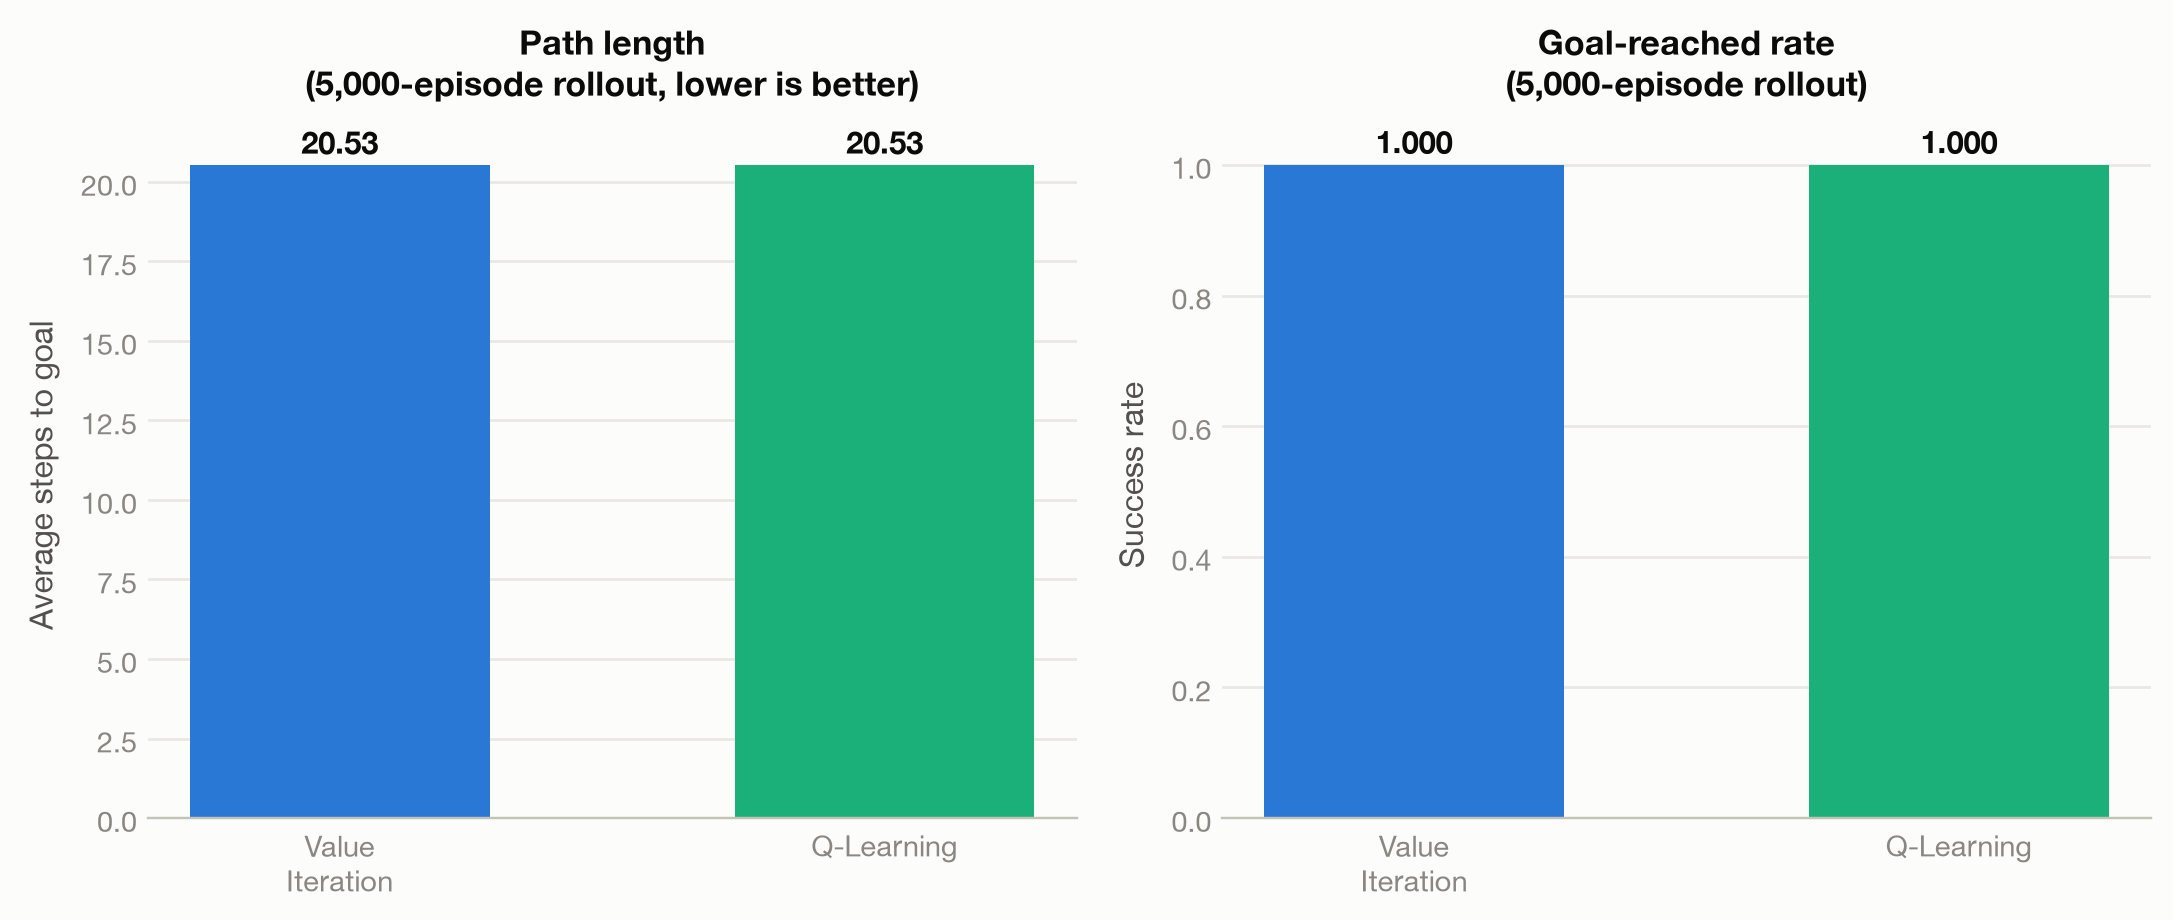
\includegraphics[width=0.85\textwidth]{fig_evaluation_comparison.png}
\caption{Performance parity: path length and success rate, 5{,}000-episode
rollouts.}
\label{fig:eval}
\end{figure}

\subsection{The policies agree almost everywhere: the optimum is not flat}

Q-Learning's greedy policy agrees with Value Iteration's exact policy on
\textbf{61 of 69} states (88.4\%), and every state is visited at
least once over 50{,}000 training episodes (Figure~\ref{fig:polagree}).
Figure~\ref{fig:gaps} shows why: the median best-vs-second-best action
margin across the MDP is 0.83, and 64 of the 69 states have a margin of at
least $0.1$. The margin only collapses toward zero at a small cluster of
low-margin states where several directions are near-equivalent because there
is no wind there to break the tie. With a clearly best action almost
everywhere, a sampling-based learner given enough episodes converges to the
same action on the vast majority of states; the eight disagreements left are
concentrated at that near-tied cluster and at states a near-optimal policy
rarely visits, which are consequently the last to be learned
(Figure~\ref{fig:polagree}).

\begin{figure}[H]
\centering
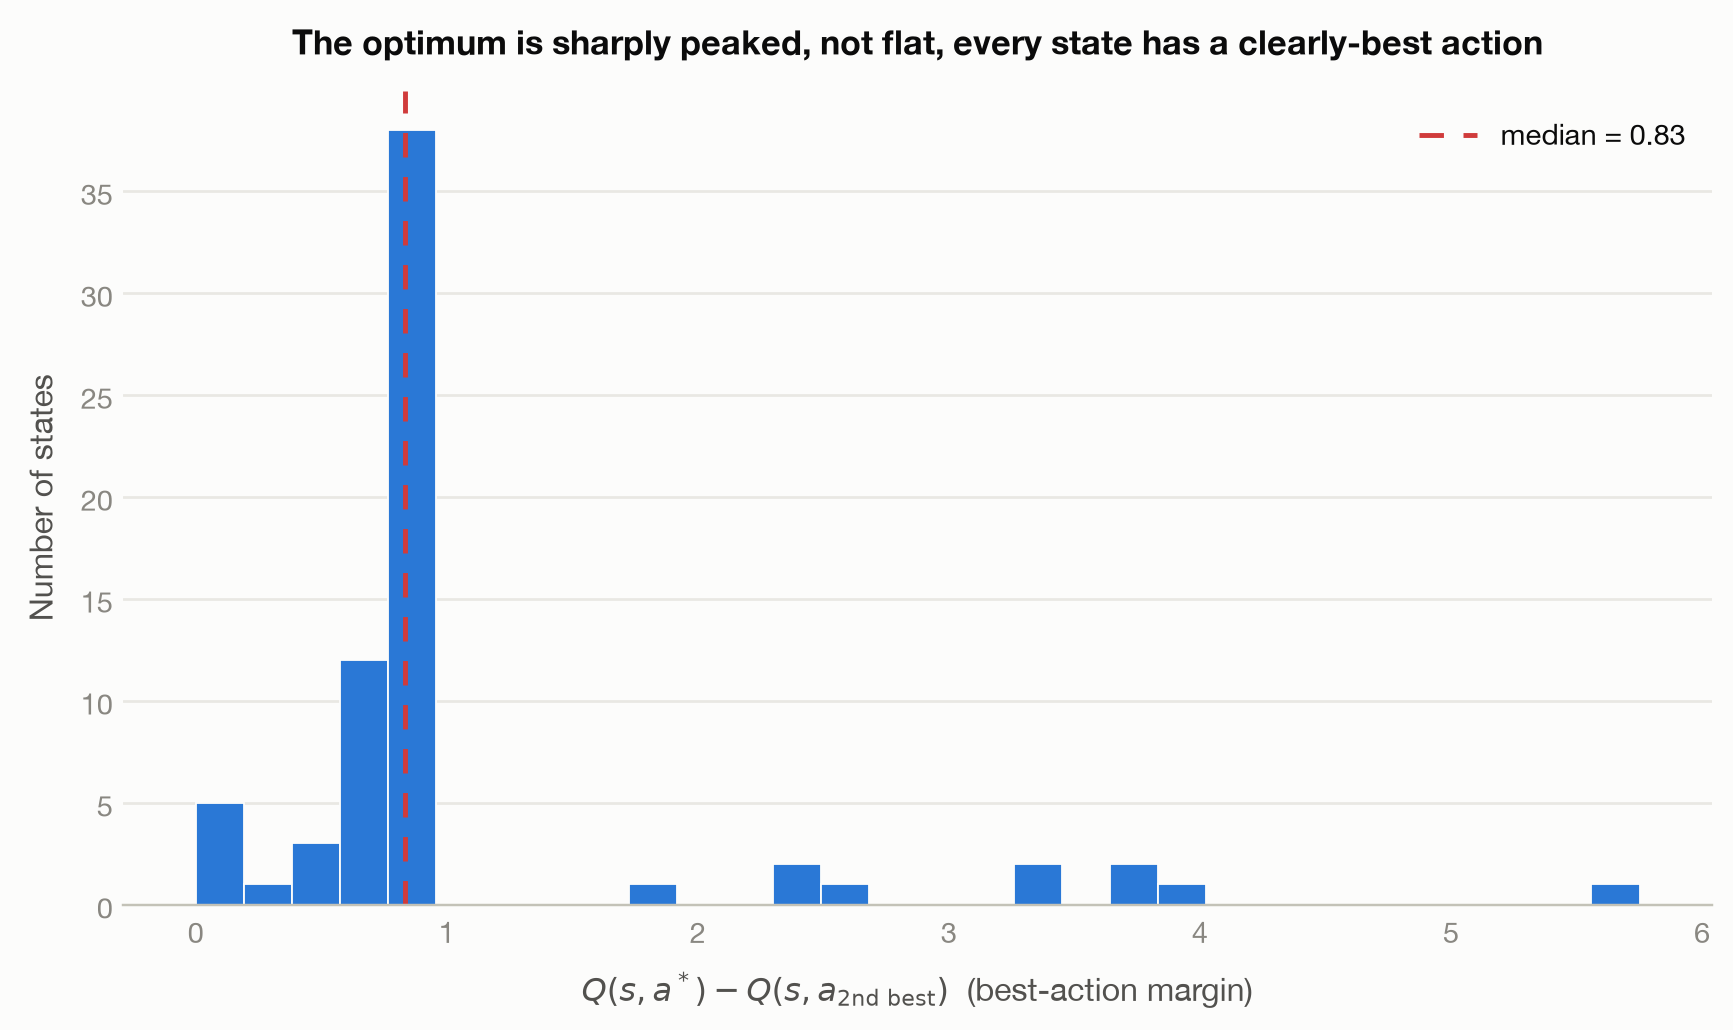
\includegraphics[width=0.6\textwidth]{fig_gaps.png}
\caption{Distribution of the best-action margin across all 69 states:
sharply peaked well above zero.}
\label{fig:gaps}
\end{figure}

\begin{figure}[H]
\centering
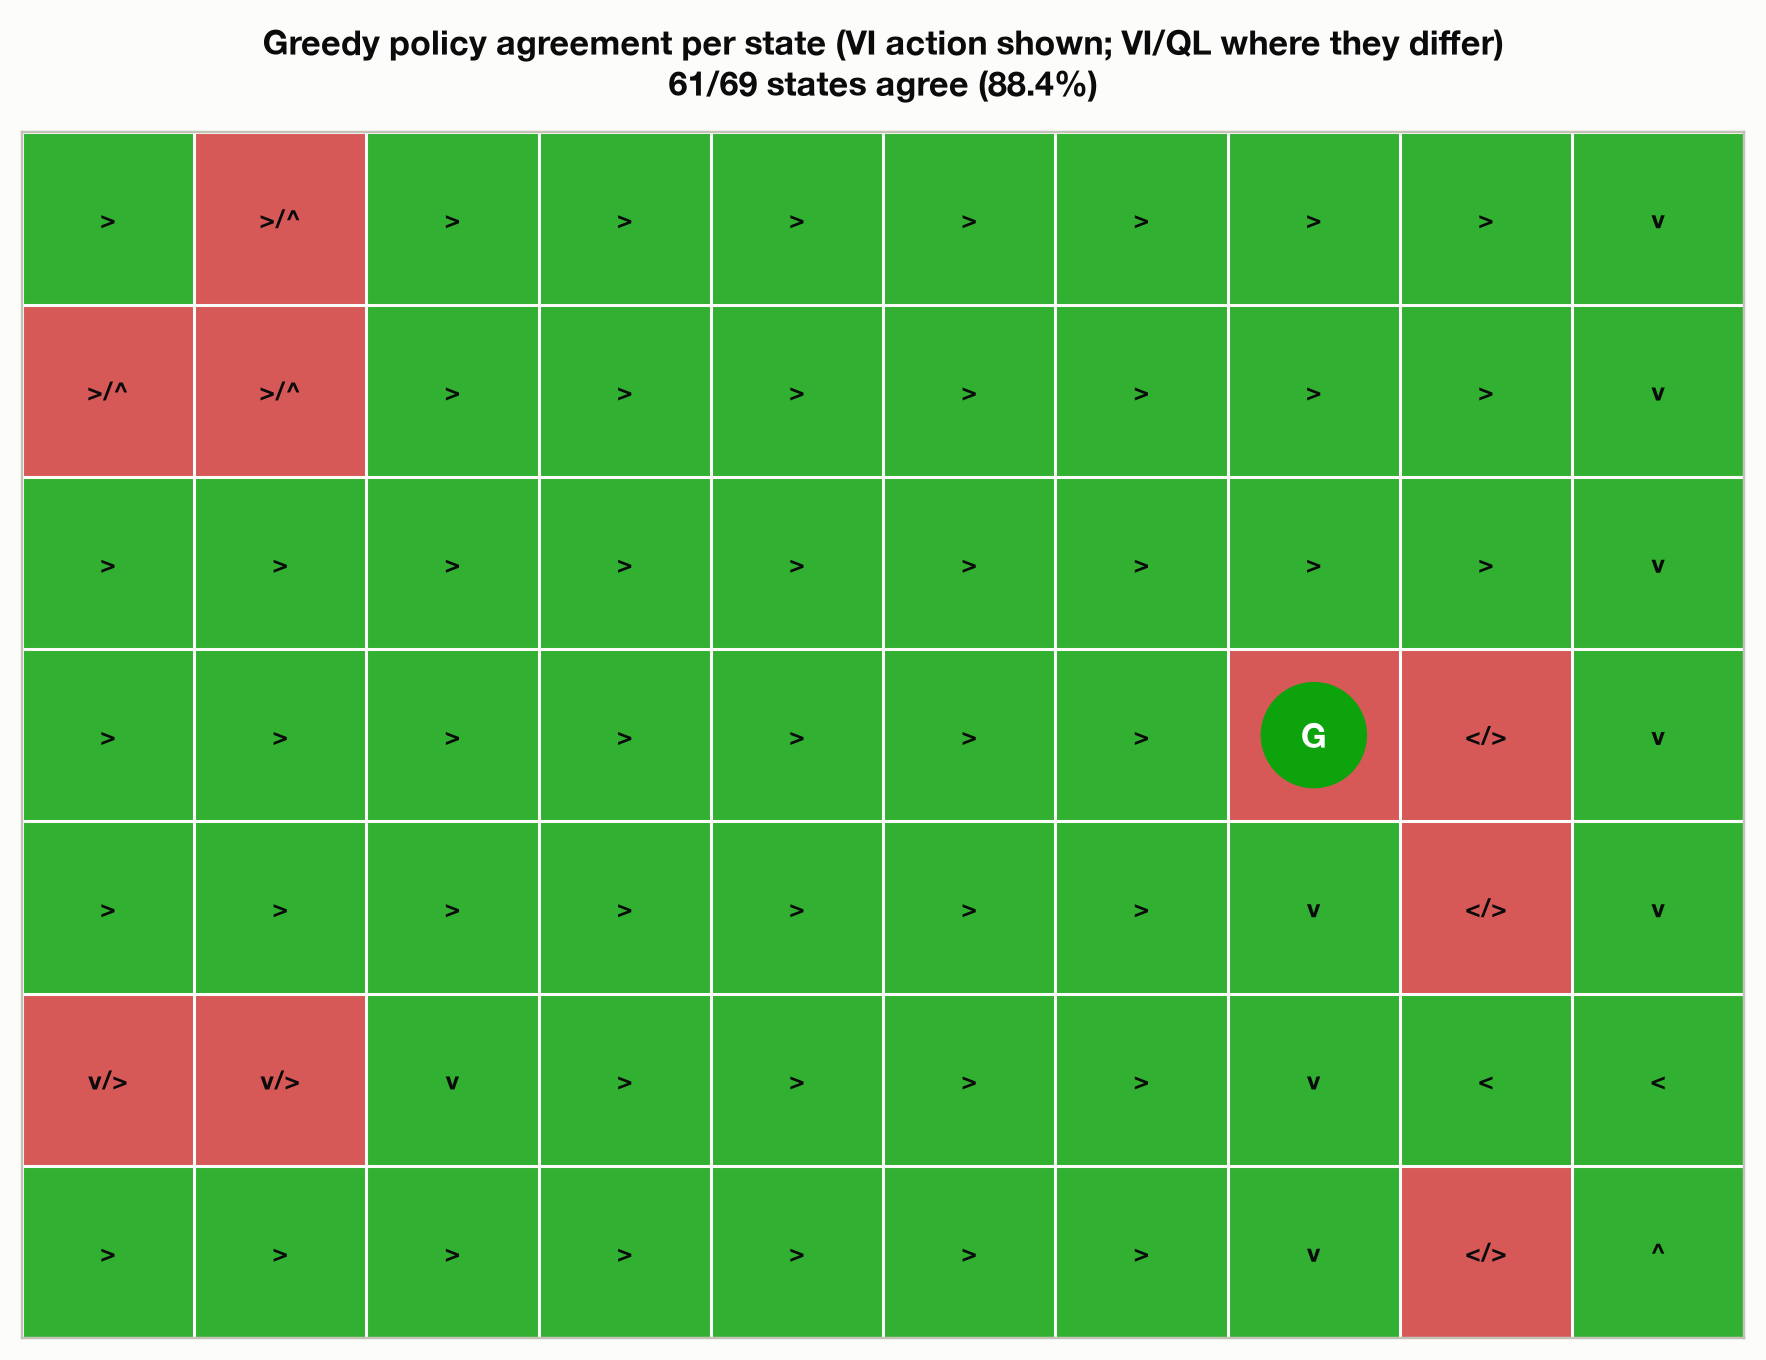
\includegraphics[width=0.78\textwidth]{fig_policy_agreement.png}
\caption{Per-state greedy action: Value Iteration's action is shown; where
Q-Learning disagrees, both are shown as VI/QL. Green = agreement, red =
disagreement among non-terminal cells; the absorbing goal (marked G) is
excluded from the 69 policy states and is not a disagreement despite its
cell shading.}
\label{fig:polagree}
\end{figure}

\begin{figure}[H]
\centering
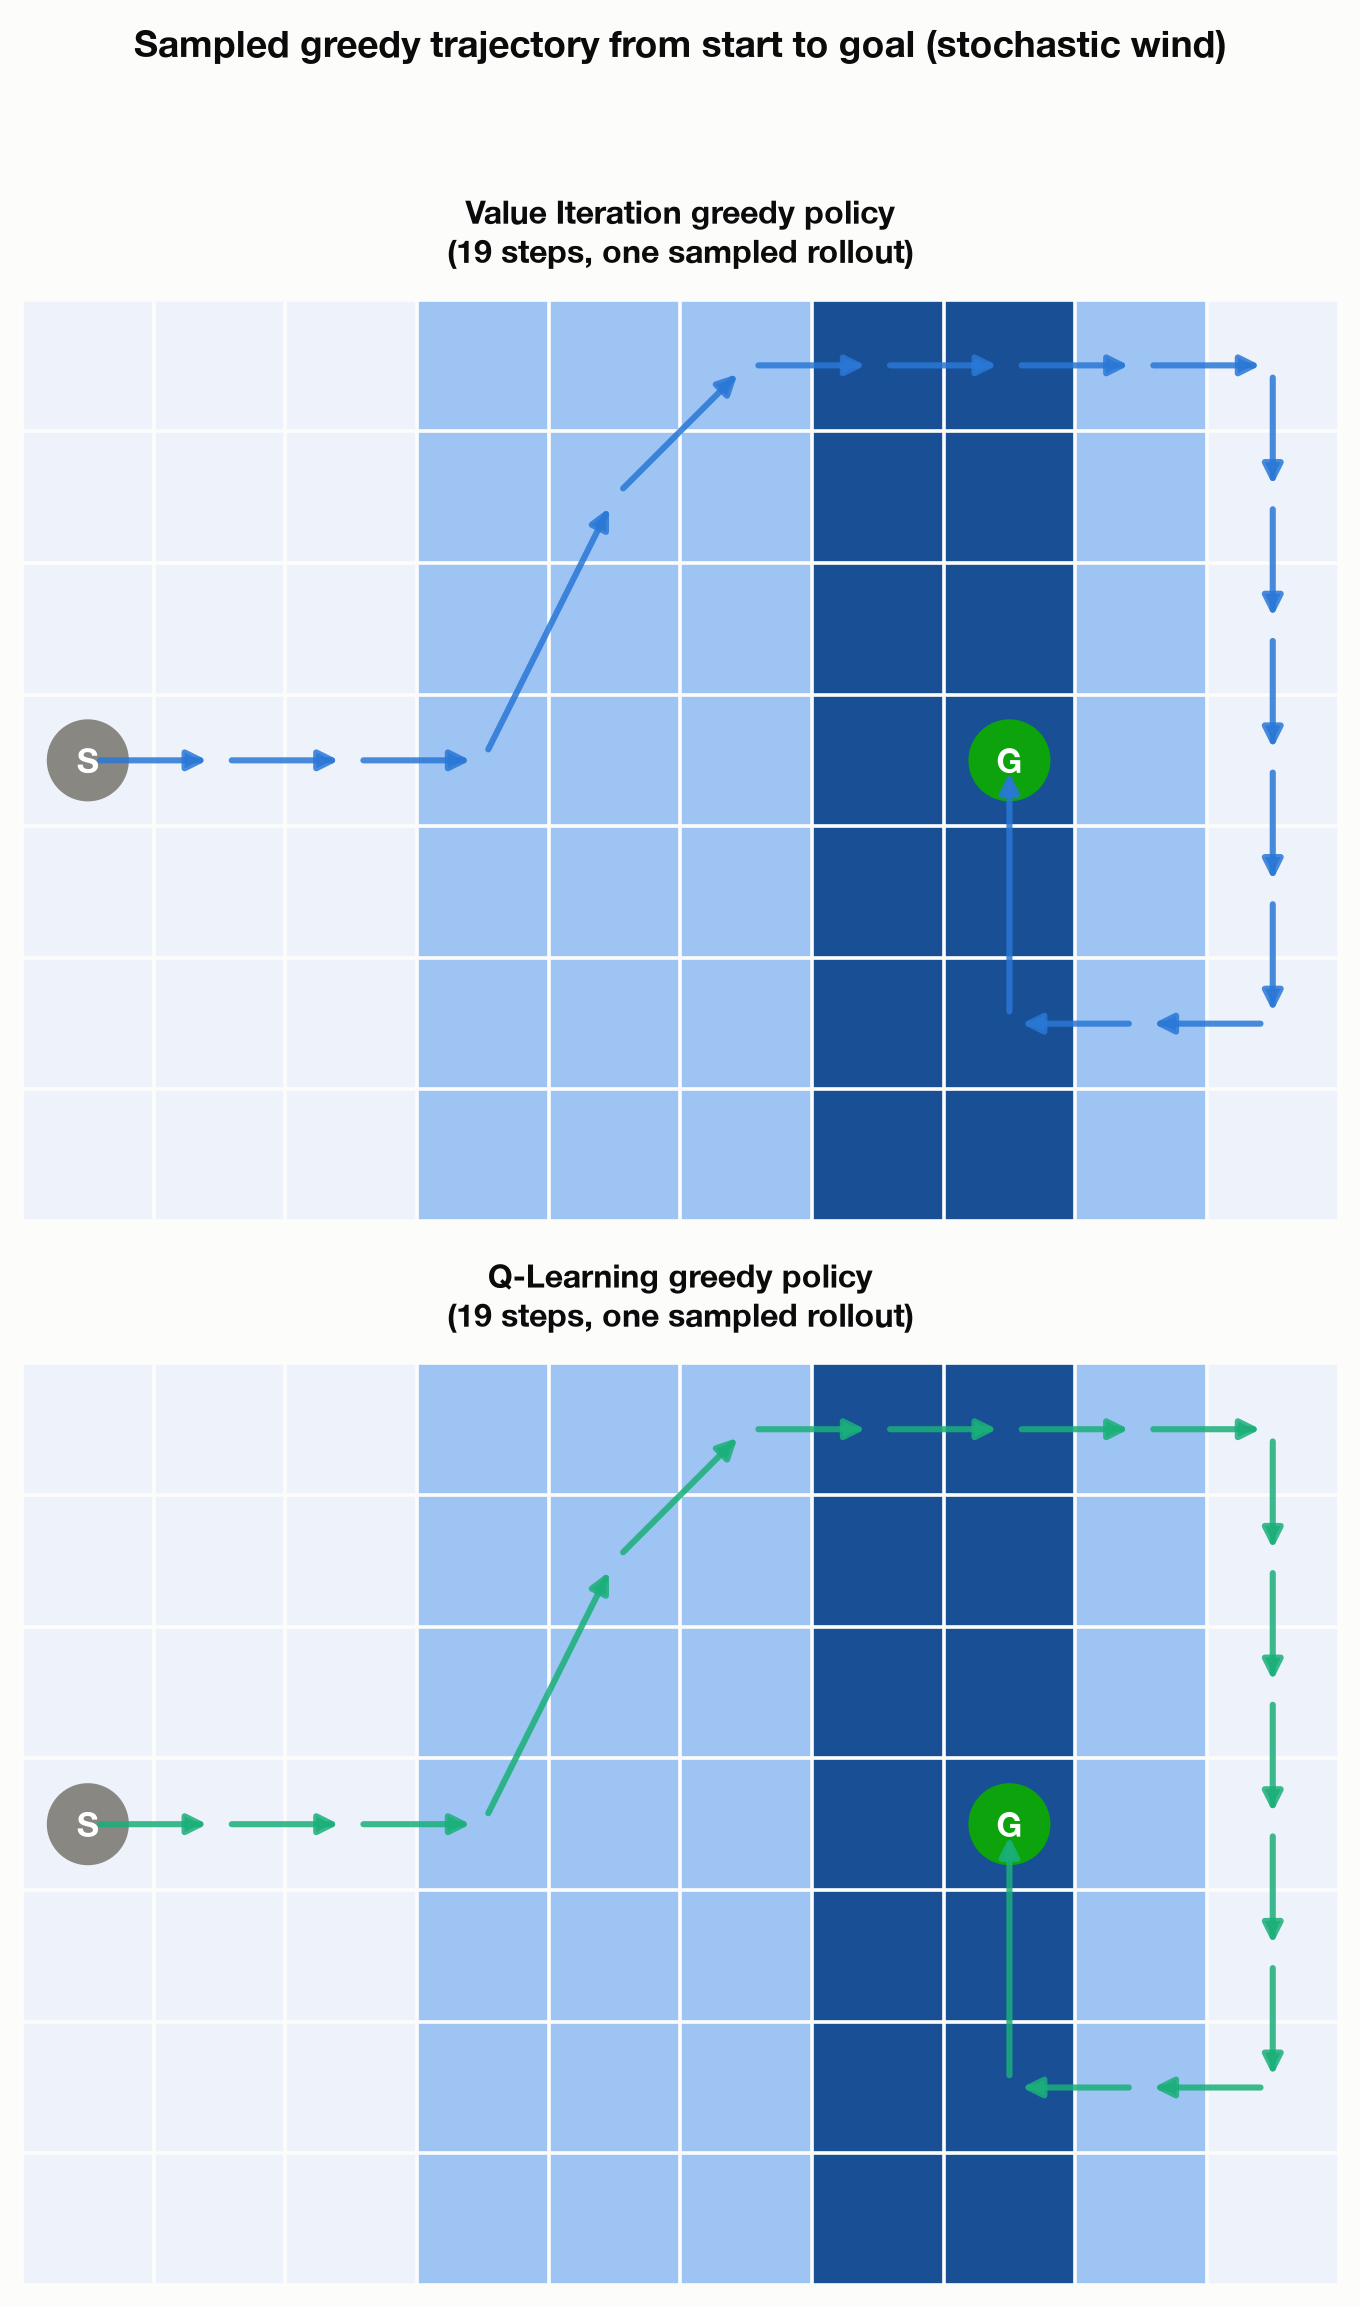
\includegraphics[width=0.62\textwidth]{fig_trajectories.png}
\caption{A single sampled greedy rollout for each policy, from the same
start under the same stochastic wind seed; both take the same route and the
same number of steps on this sample.}
\label{fig:traj}
\end{figure}

\section{Hyperparameter Experiments}

\subsection{Discount factor changes the policy, not only convergence speed}

Figure~\ref{fig:gamma} sweeps $\gamma\in\{0.7,0.9,0.95,0.99,1.0\}$. For
$\gamma\ge0.95$ the greedy average path length is flat at 20.37 steps,
effectively the same policy. Lowering
$\gamma$ further changes the policy more substantially: at $\gamma=0.9$,
6 of 69 states switch their optimal action and average path length
rises to 21.37 steps; at $\gamma=0.7$, 13 of 69 states
differ and path length rises to 27.75 steps. This matches the prediction of
Section~3: because a smaller $\gamma$ discounts distant steps much more
heavily, the objective is no longer a good proxy for raw expected step count
once the wind's stochastic branching is in play, and Value Iteration finds a
policy that is worse in expectation under the undiscounted metric even
though it is optimal for the smaller-$\gamma$ objective it was asked to
solve. This effect would not occur in the corresponding deterministic
constant-step-cost shortest-path formulation; Windy Gridworld's real
stochasticity is what produces it. (The sweep's $\gamma=1.0$ point is
undiscounted: the return there is interpreted by its limit as $-T$ and does
not inherit the usual discounted Bellman-contraction guarantee assumed for
$\gamma\in(0,1)$ elsewhere in this section.)

\begin{figure}[H]
\centering
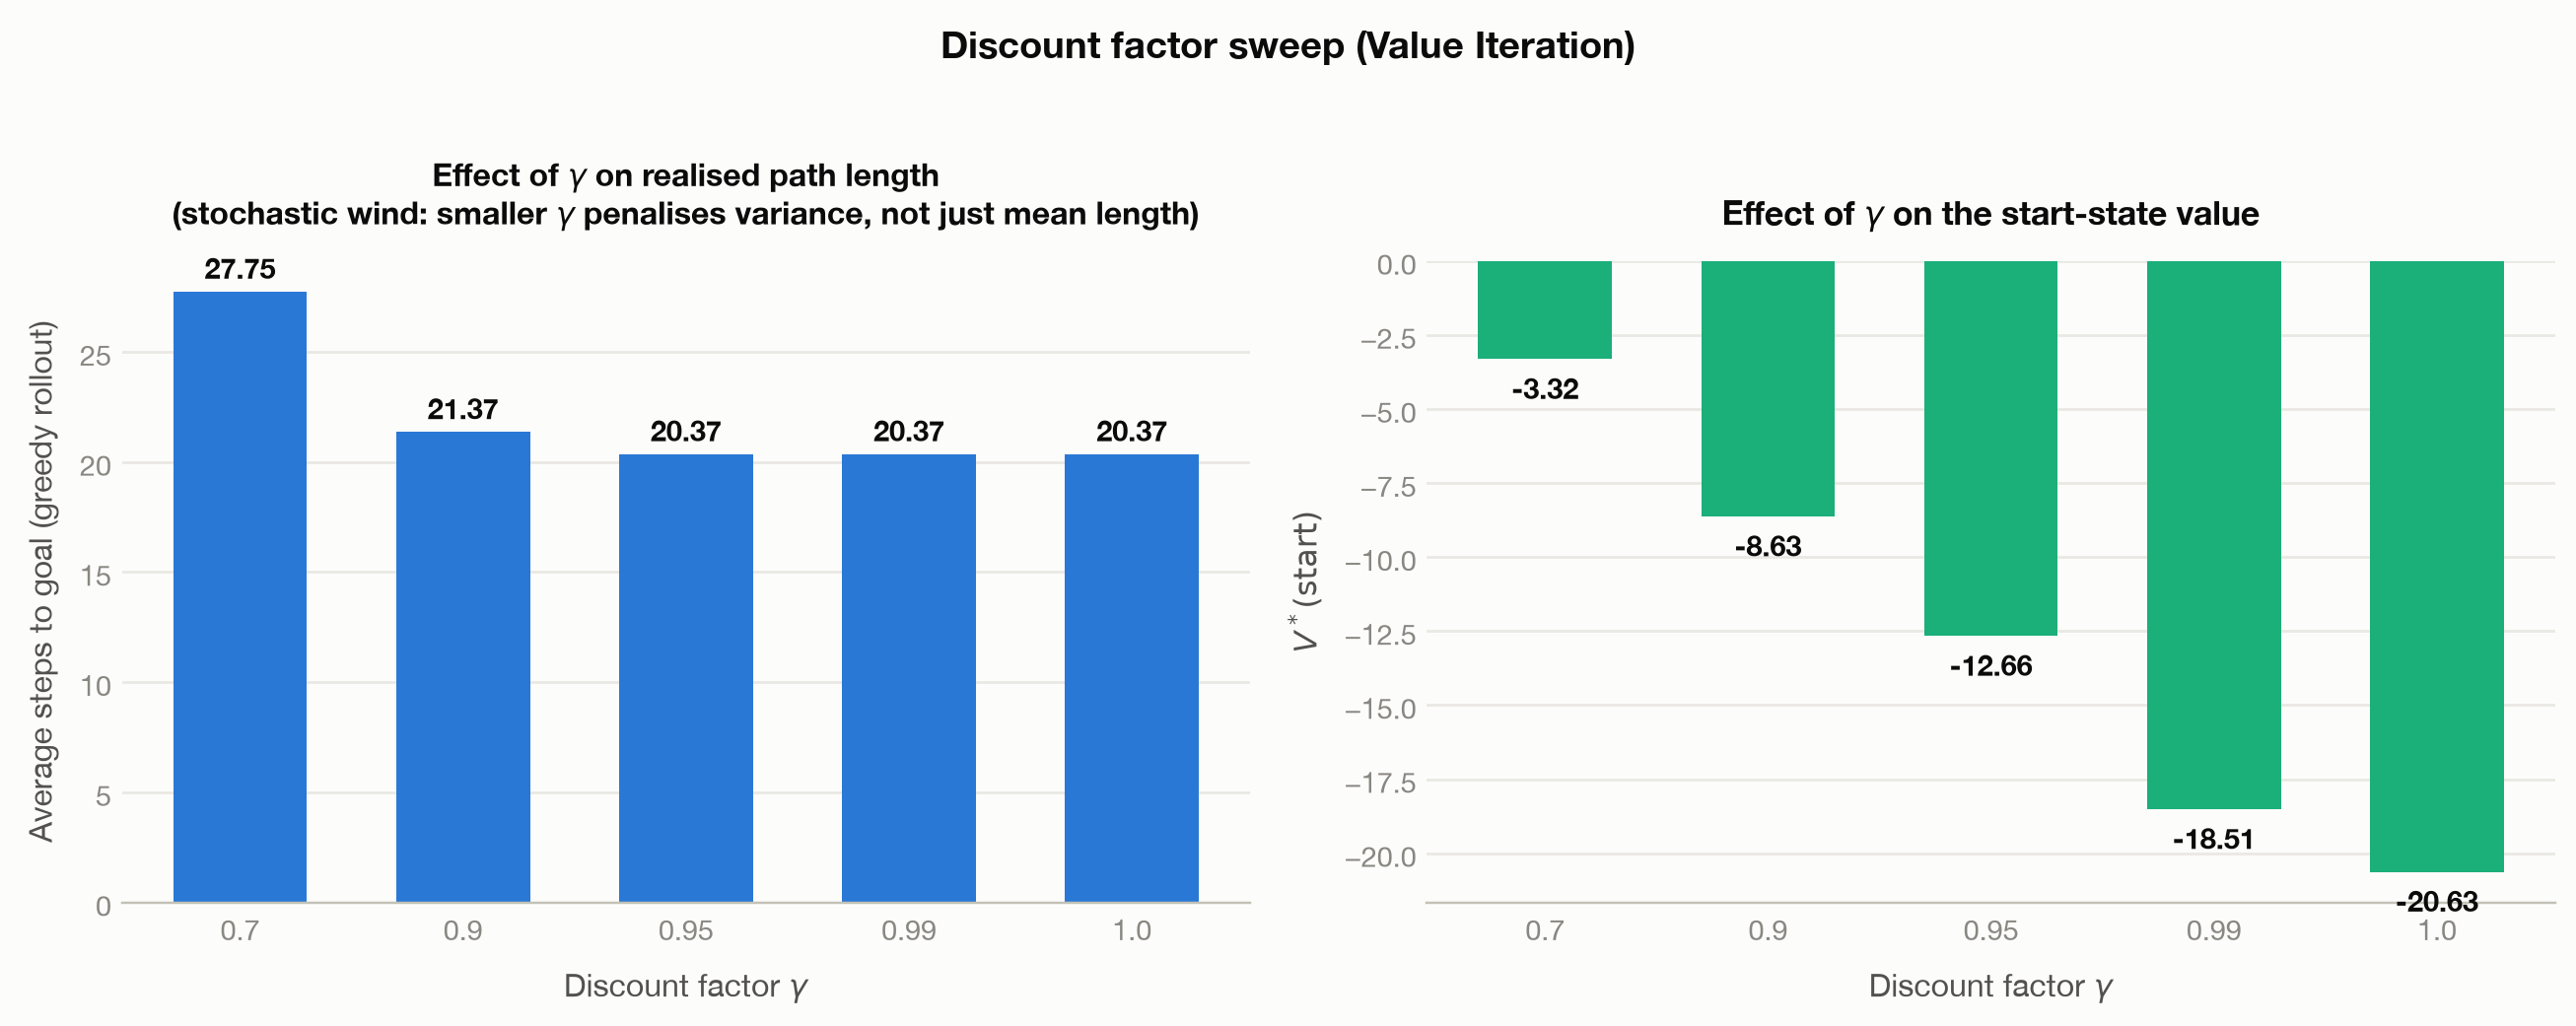
\includegraphics[width=0.85\textwidth]{fig_gamma_sweep.png}
\caption{Discount factor sweep: realised path length is flat for
$\gamma\ge0.95$ but rises as $\gamma$ drops to 0.9 and 0.7, where 6 and 13
states' optimal actions respectively actually change.}
\label{fig:gamma}
\end{figure}

\subsection{Stopping threshold: cost without benefit, here}

Value Iteration's other named hyperparameter is the stopping threshold
$\theta$: the sweep terminates once the maximum change in $V$ across all
states drops below $\theta$. Figure~\ref{fig:theta} sweeps six values of
$\theta$ from $10^{-2}$ down to $10^{-12}$ at $\gamma=0.99$. The cost side
follows the Bellman contraction directly: tightening $\theta$ by two orders
of magnitude costs a roughly fixed number of extra sweeps (36, 56, 76, 96,
116, 136), an arithmetic rather than exponential progression, since each
sweep shrinks the remaining error by the fixed factor $\gamma=0.99$. The
benefit side is flat: comparing every $\theta$'s greedy policy against the
tightest run ($\theta=10^{-12}$) gives 100\% agreement at every tested
value, including the loosest $\theta=10^{-2}$. In this MDP the greedy policy
was unchanged for every tested threshold, including $\theta=10^{-2}$.
Unlike $\gamma$, which changes \emph{which} policy is optimal
(Section~8.1), $\theta$ only trades sweeps for numerical precision that this
task does not need; the default $\theta=10^{-10}$ used elsewhere in this
report is more than tight enough, though a much looser value would have
given the identical policy for a third of the sweeps.

\begin{figure}[H]
\centering
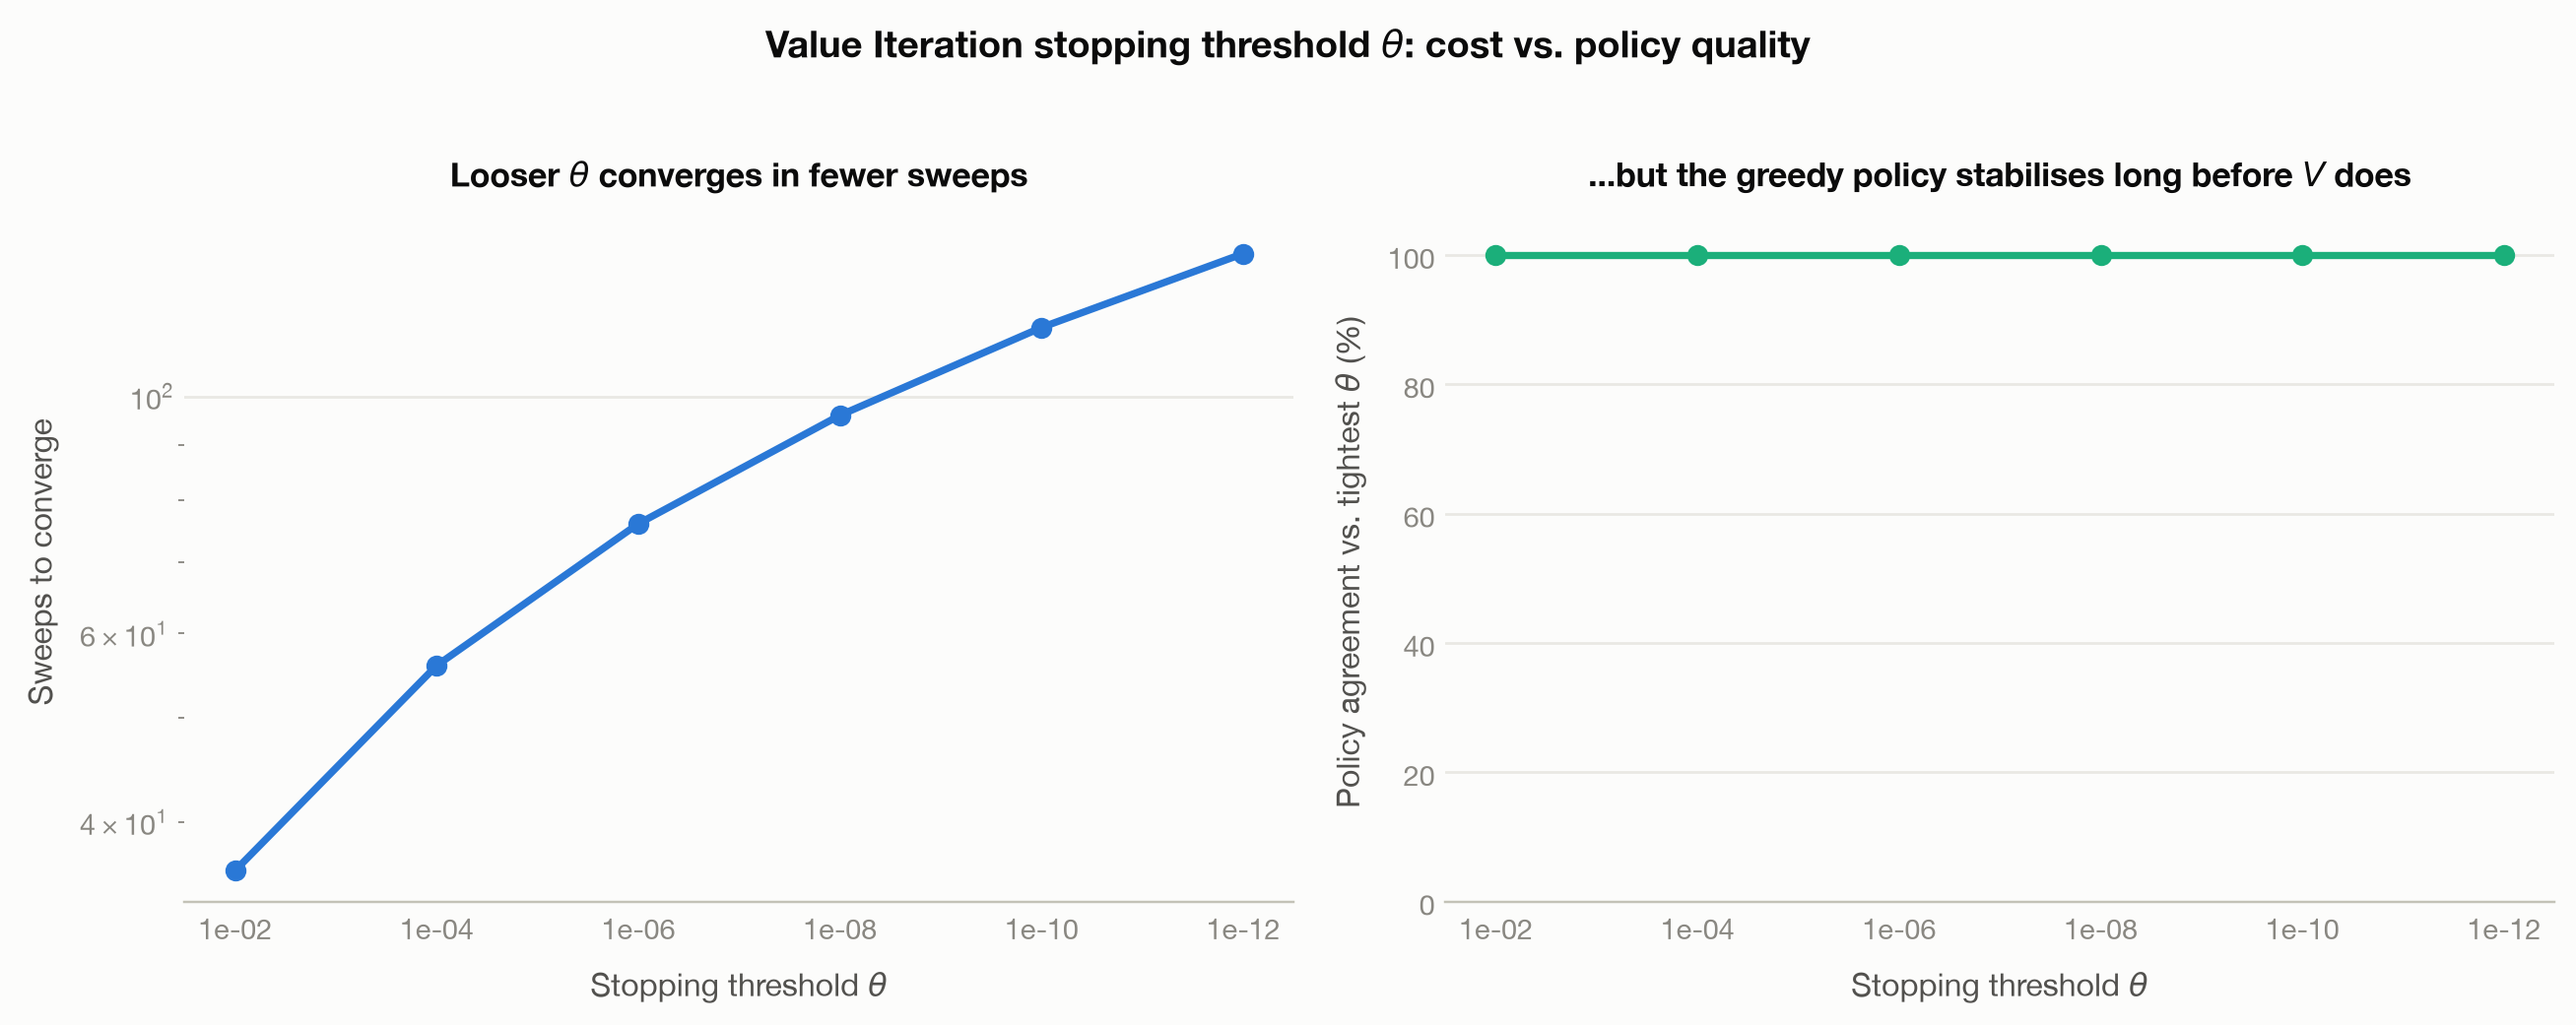
\includegraphics[width=0.85\textwidth]{fig_theta_sweep.png}
\caption{Stopping-threshold sweep: sweeps-to-converge rises steadily as
$\theta$ tightens (left), while the resulting greedy policy is identical to
the tightest-$\theta$ policy at every setting tested (right).}
\label{fig:theta}
\end{figure}

\subsection{Learning rate and exploration decay}

Figure~\ref{fig:alpha} sweeps Q-Learning's learning rate over the exact set
$\alpha\in\{0.02,0.05,0.1,0.3,0.5\}$. All
settings converge toward Value Iteration's optimum; smaller $\alpha$
($0.02$--$0.1$) converges to a slightly lower, steadier plateau, while larger
$\alpha$ ($0.3$--$0.5$) is noisier and settles a little above the optimum,
the familiar bias/variance trade-off of the running average that a Q-value
update performs. The exploration-decay sweep
(Figure~\ref{fig:epsilon}) uses the multiplicative schedule
$\varepsilon_t=\max(0.02,\,\varepsilon_0 d^{\,t})$ with
$d\in\{0.999,0.9999,0.99995\}$, and shows the same overall pattern: decaying
$\varepsilon$ too fast ($d=0.999$) starves the
agent of the exploration it needs to discover the shorter route around the
wind, while a slower decay ($d=0.99995$) reaches the optimum in more episodes but more
reliably. Both sweeps train for the same 50{,}000 episodes as the main
Q-Learning run above, each setting as a single run with seed 42 rather than
an average over multiple seeds, and both figures plot a 100-episode moving
average of steps to goal.

\begin{figure}[H]
\centering
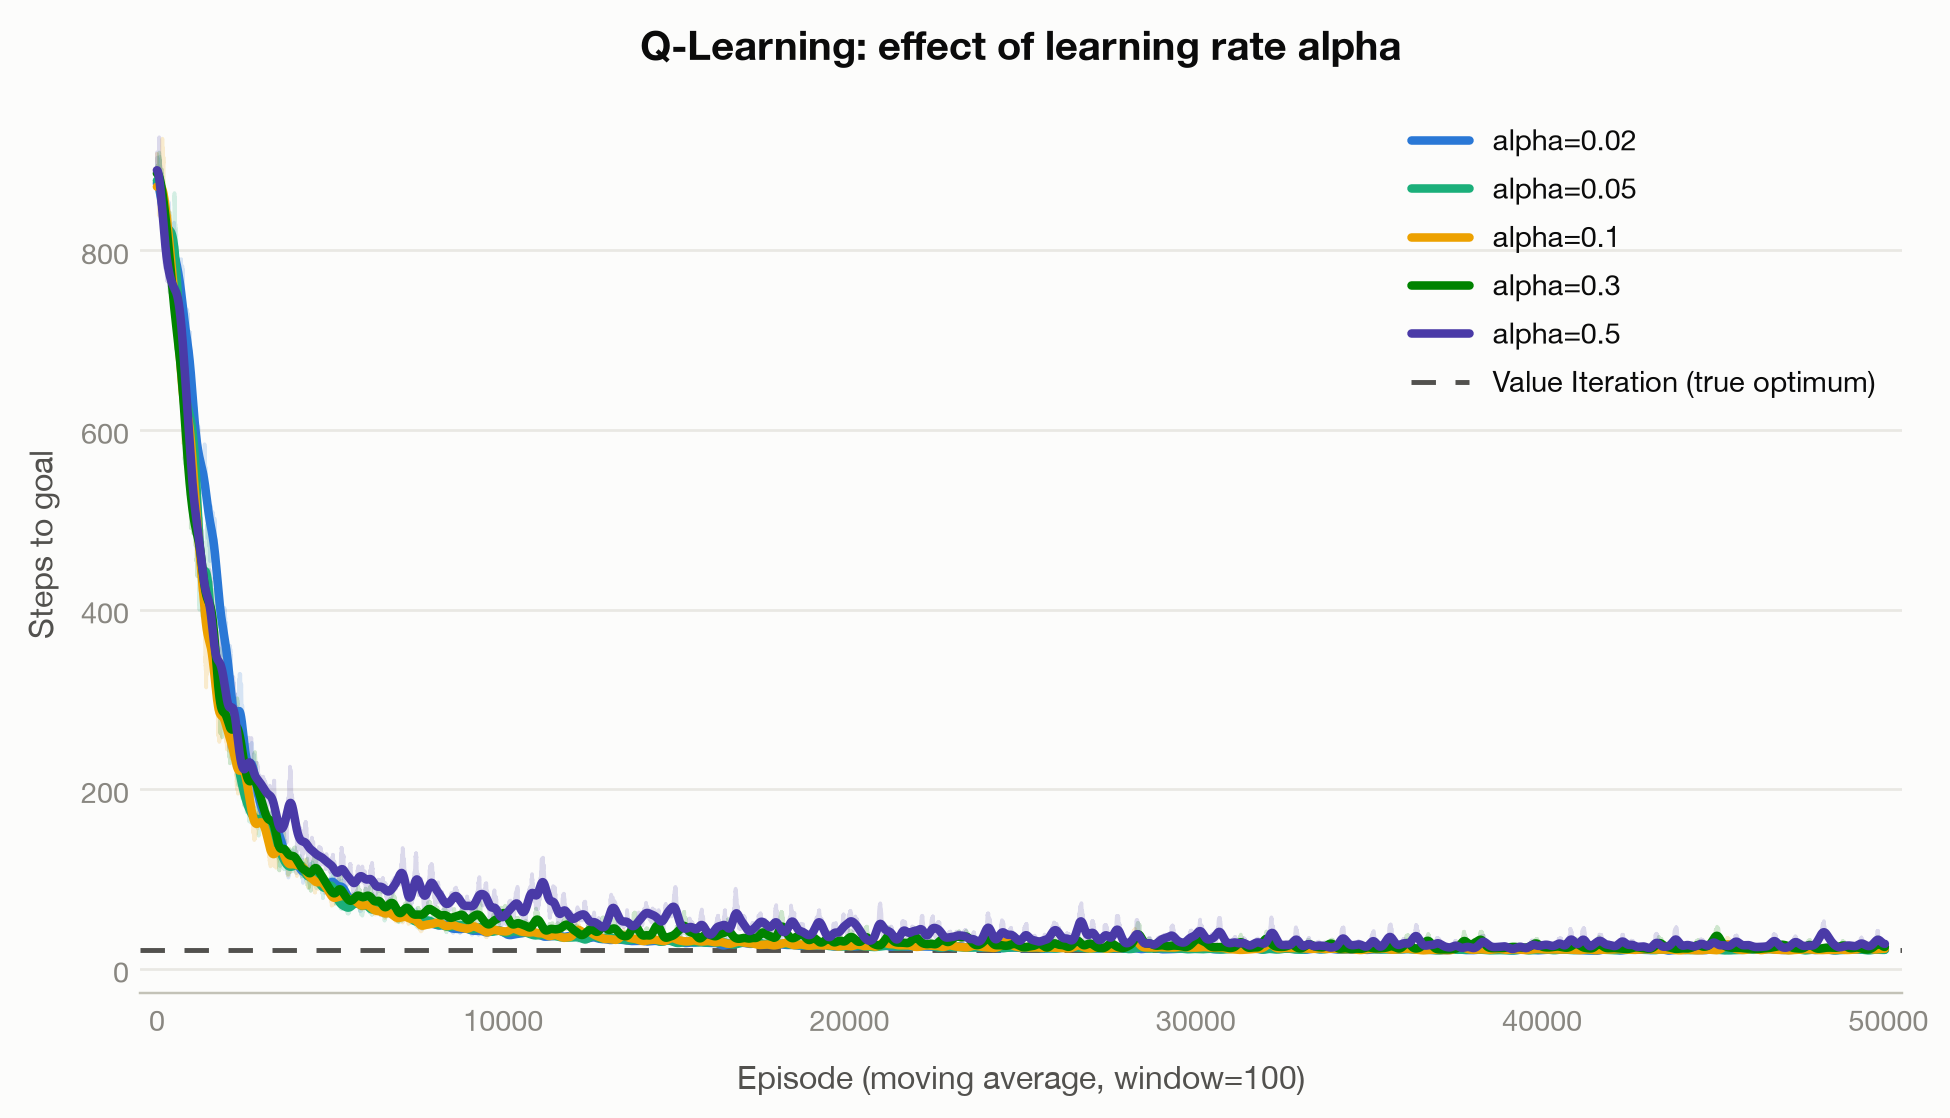
\includegraphics[width=0.82\textwidth]{fig_alpha_sweep.png}
\caption{Effect of the learning rate on Q-Learning's convergence toward
Value Iteration's optimum (lower is better).}
\label{fig:alpha}
\end{figure}

\begin{figure}[H]
\centering
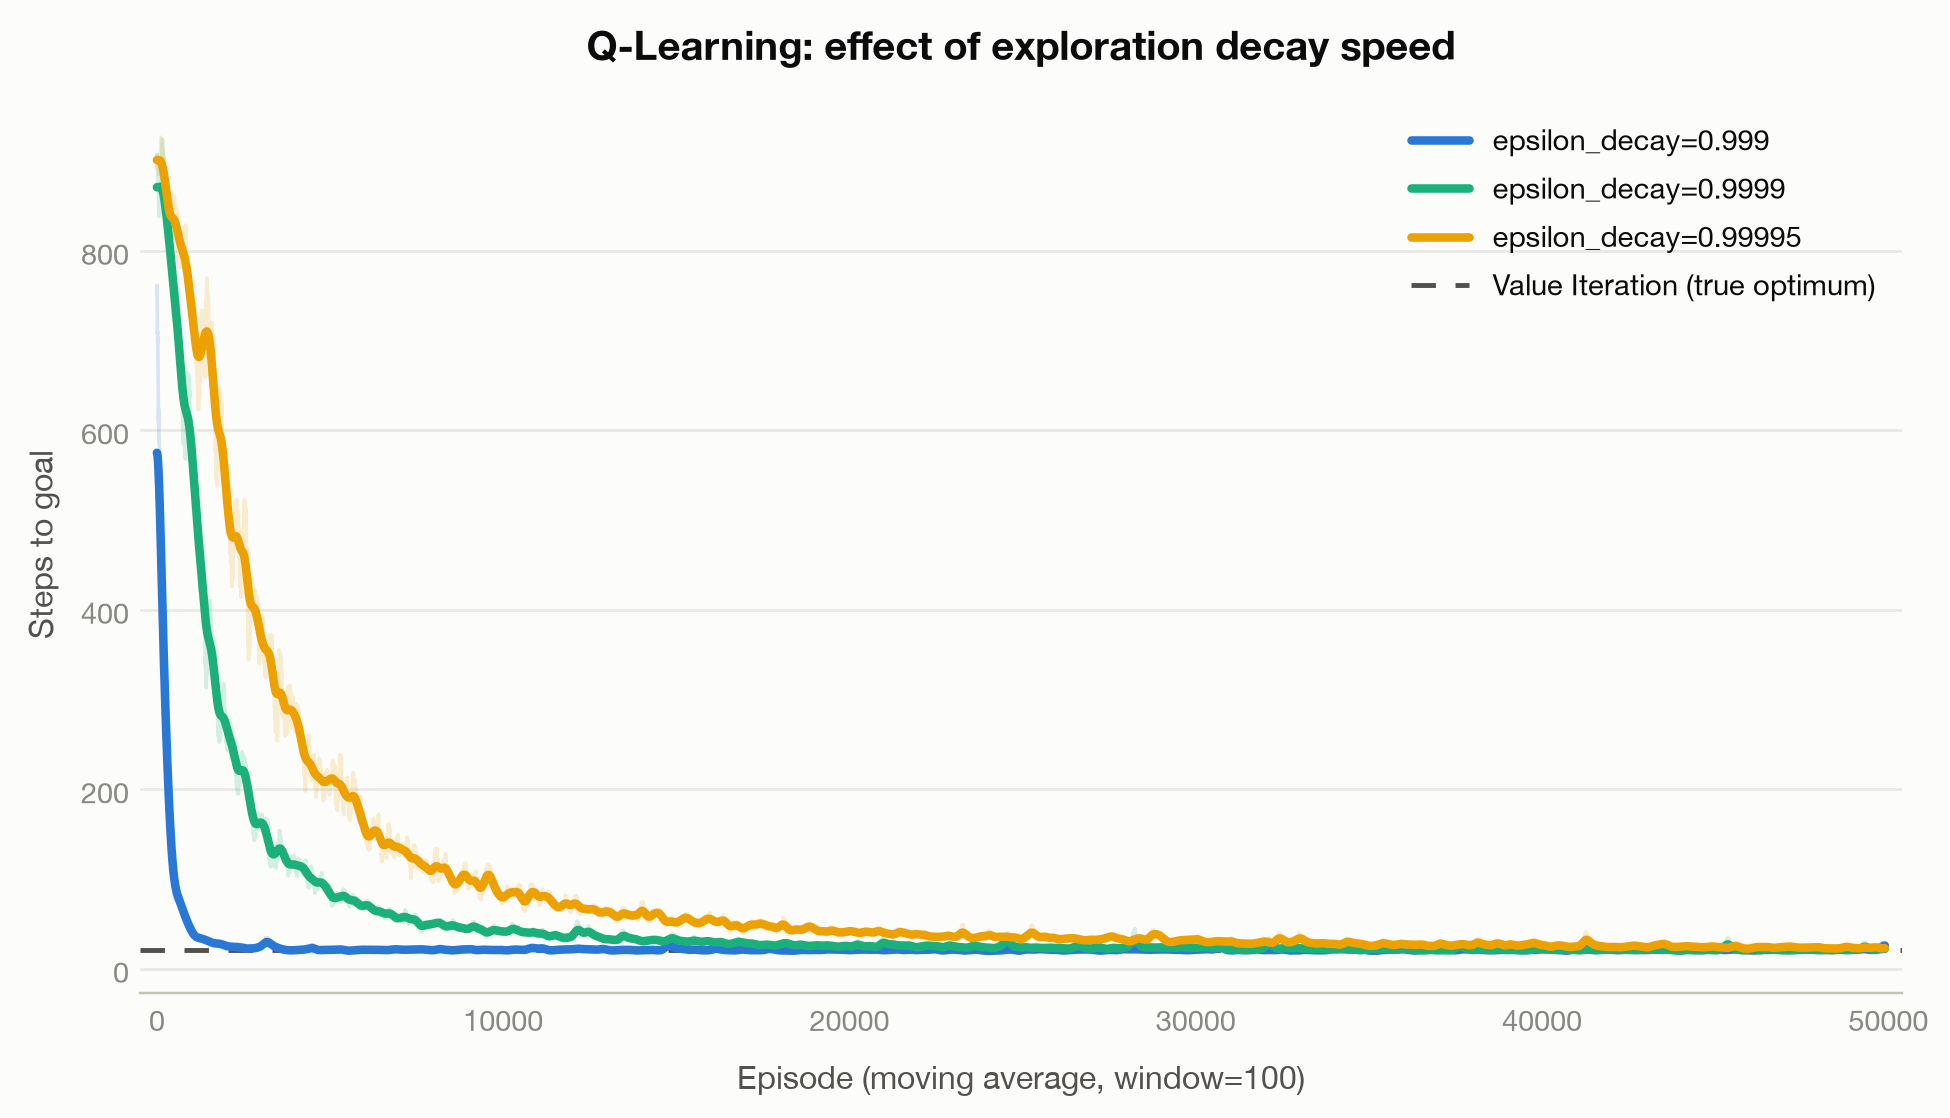
\includegraphics[width=0.82\textwidth]{fig_epsilon_sweep.png}
\caption{Effect of the exploration-decay rate on Q-Learning's convergence
toward Value Iteration's optimum (lower is better).}
\label{fig:epsilon}
\end{figure}

\section{Model-Based vs.\ Model-Free}

\begin{table}[H]
\centering
\caption{Model-based vs.\ model-free on the Stochastic Windy Gridworld.}
\label{tab:tradeoffs}
\small
\begin{tabularx}{\textwidth}{@{}p{3.8cm}XX@{}}
\toprule
 & Value Iteration (model-based) & Q-Learning (model-free) \\
\midrule
Needs a transition model & Yes: derived from the wind's known probabilities & No: only \texttt{env.step()} \\
Environment interactions & 0 & 50{,}000 episodes ($\sim$20 steps each) \\
Recovers the exact policy & Yes (exact expectations) & Yes, on 88.4\% of states; the optimum is not flat, so sampling suffices \\
Rollout performance & 20.53 avg.\ steps & 20.53 avg.\ steps on a separate evaluation batch \\
Sensitive to $\gamma$'s exact value & Yes: changes the policy under real stochasticity & Not separately tested; Q-Learning optimizes the same discounted objective \\
Sensitive to $\theta$'s exact value & No: identical policy across all tested $\theta$ (Section~8.2) & N/A: has no stopping threshold \\
\bottomrule
\end{tabularx}
\end{table}

With a stochastic environment and a sharply-peaked (non-flat) optimum,
Q-Learning matches Value Iteration's performance and recovers nearly the
same policy, state by state, with no model and no access to the wind's
probabilities. The remaining disagreements are the rarely-visited states
any sample-based method would learn last. The fundamental trade-off between
the two methods is a model bought with derivation effort and zero
environment interaction, versus tens of thousands of real episodes needed
to learn from scratch.

\section{Conclusion}

A transition model for the Stochastic Windy Gridworld was derived
analytically from the wind's known probabilities and solved exactly with
Value Iteration in 116 sweeps, reaching the goal in 20.53 steps on average.
Q-Learning, trained without any model for 50{,}000 episodes, produced
approximately the same rollout performance (20.53 steps, on a separate
evaluation batch) and recovered the \emph{same}
greedy policy on 88.4\% of states. This follows from the MDP's mostly
sharply-peaked optimum: 64 of 69 states have an action-value margin of at
least 0.1. The discount-factor sweep showed that, because the wind makes
the environment stochastic, $\gamma$ does more than guarantee convergence:
dropping $\gamma$ from 0.99 to 0.9 or 0.7 changes the optimal action at 6 and
13 states respectively. The stopping threshold $\theta$, Value Iteration's
other named hyperparameter, only traded sweeps for numerical precision this
task did not need: the greedy policy was identical across six orders of
magnitude of $\theta$. Windy Gridworld's combination of genuine stochasticity
and a sharply-peaked optimum is exactly what lets model-free learning
recover both the model-based performance and the model-based policy.

\end{document}
